\documentclass{standalone}

\usepackage{tikz}
\usepackage{tikz-qtree}
\usepackage{../../../texmf/tex/latex/mathoperators/mathoperators}

%TODO how to do two or three trees next to eatch other
% https://tex.stackexchange.com/questions/258850/putting-a-tree-next-to-another-tree

\begin{document}
	\begin{
	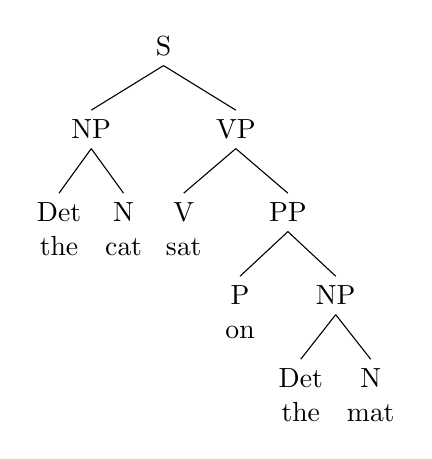
\begin{tikzpicture}
	\tikzset{every tree node/.style={align=center,anchor=north}}
	\Tree [.S [.NP Det\\the N\\cat ]
	[.VP V\\sat
	[.PP P\\on
	[.NP Det\\the N\\mat ] ] ] ]
	\end{tikzpicture}
\end{document}